\twocolumn[\begin{@twocolumnfalse}
	\chapter{Making a Network Adaptor cable\hfill\difficulty{3}}
	The NABU Network Adaptor is the interface between the NABU Personal Computer and the cable television network that enables software applications and other digital data to be downloaded from NABU's back-end systems. The NABU Preservation Project has released an Internet Adaptor\footnotemark, which emulates the NABU Network Adaptor, allowing a NABU PC to download applications and data via the Internet. This section describes how to create a DB-9 to DIN-5 adaptor cable that allows a NABU PC to be connected via RS-422 to a system running the Internet Adaptor software. If required, a RS-422 interface can easily be added to the system hosting the Internet Adapter by means of a USB to RS-422 adaptor.
	\vskip1em
\end{@twocolumnfalse}]
\footnotetext[1]{See the NABU RetroNet website <https://nabu.ca> for details.}

\section{Network Adaptor cable wiring}
The \texttt{ADAPTOR} port on the back of the NABU Personal Computer implements a full-duplex RS-422 interface, which requires 4 wires for communication between devices. Because of the high transmission (baud) rates involved, a twisted-pair shielded cable is highly recommended for the DB-9 to DIN-5 adaptor (as per the RS-422 standard). Category 5 cable (as used in Ethernet cabling) is available both as shielded twisted pair and as unshielded twisted pair and generally exceeds the recommendations for RS-422, making it an excellent choice --- if no twisted pair cable is available, the length of the adaptor cable \textit{must} be kept as short as possible, and should not exceed 6-8 inches. When using shielded cable, the shielding must only be connected to one of the connectors to avoid a ground loop.

The cable must be wired as specified in Table~\ref{tbl:adaptor}. If at all possible, use twisted-pair cable and group the pairs as shown.

\begin{center}
	\sffamily
	\begin{tblr}{
			colspec={r|cccc|},
			cell{1}{2} = {c=2}{c},
			cell{1}{4} = {c=2}{c},
			row{1} = {font=\bfseries},
			row{1,2} = {bg=gray4,fg=white},
			row{5,6} = {bg=gray9},
			cell{1}{1} = {r=2}{bg=white},
			cell{3}{1} = {r=2}{},
			cell{5}{1} = {r=2}{},
			vline{4} = {3-6}{text=\clap{$\leftrightarrow$}},
			vline{1} = {3-6}{solid},
			hline{1} = {2-5}{solid},
			hline{3,7} = {solid}
		}
		& NABU (DIN5) & & RS-422 (DB9)\footnotemark[2] &\\
		& Signal & Pin & Pin & Signal \\
		\rotatebox{90}{Pair 1} & RXD+ & 1 & 1 & T/R+ \\
		& RXD-- & 4 & 2 & T/R-- \\
		\rotatebox{90}{Pair 2} & T/R+ & 5 & 3 & RXD+ \\
		& T/R-- & 3 & 4 & RXD-- \\
	\end{tblr}
	\taskLbl{tbl:adaptor}
	\taskTable{Adaptor cable wiring.}
\end{center}
\footnotetext[2]{Pin numbers shown are for the DTECH DT-5019 USB TO RS485/422 adaptor cable.  Refer to the relevant manufacturer's documentation for other RS-422 interfaces.}

\section{DIN-5 end of the cable}
\awesomebox[red]{2pt}{\faHandPaper}{red}{To avoid a ground loop, the cable shield should only ever be connected to ground at one end of the cable; \textit{never} at both ends. Thus, if the cable shield is connected to ground at the \mbox{RS-422} adaptor end, do \textit{not} also connect the shield to the outer rim of the DIN connector, or vice versa.}
\begin{enumerate}
	\item To minimise the number of connections that need to be soldered, a MIDI cable may be used. Alternatively, solder the pins of a \underline{male} DIN-5 connector as shown in Figure \ref{fig:din5}. Note that the pin numbers shown in the diagram are for the solder side of the connector. Also note that the \mbox{DIN-5} connector pins are not numbered sequentially.
\end{enumerate}

\begin{figure}[t!]
	\begin{center}
		\scalebox{0.175}{
			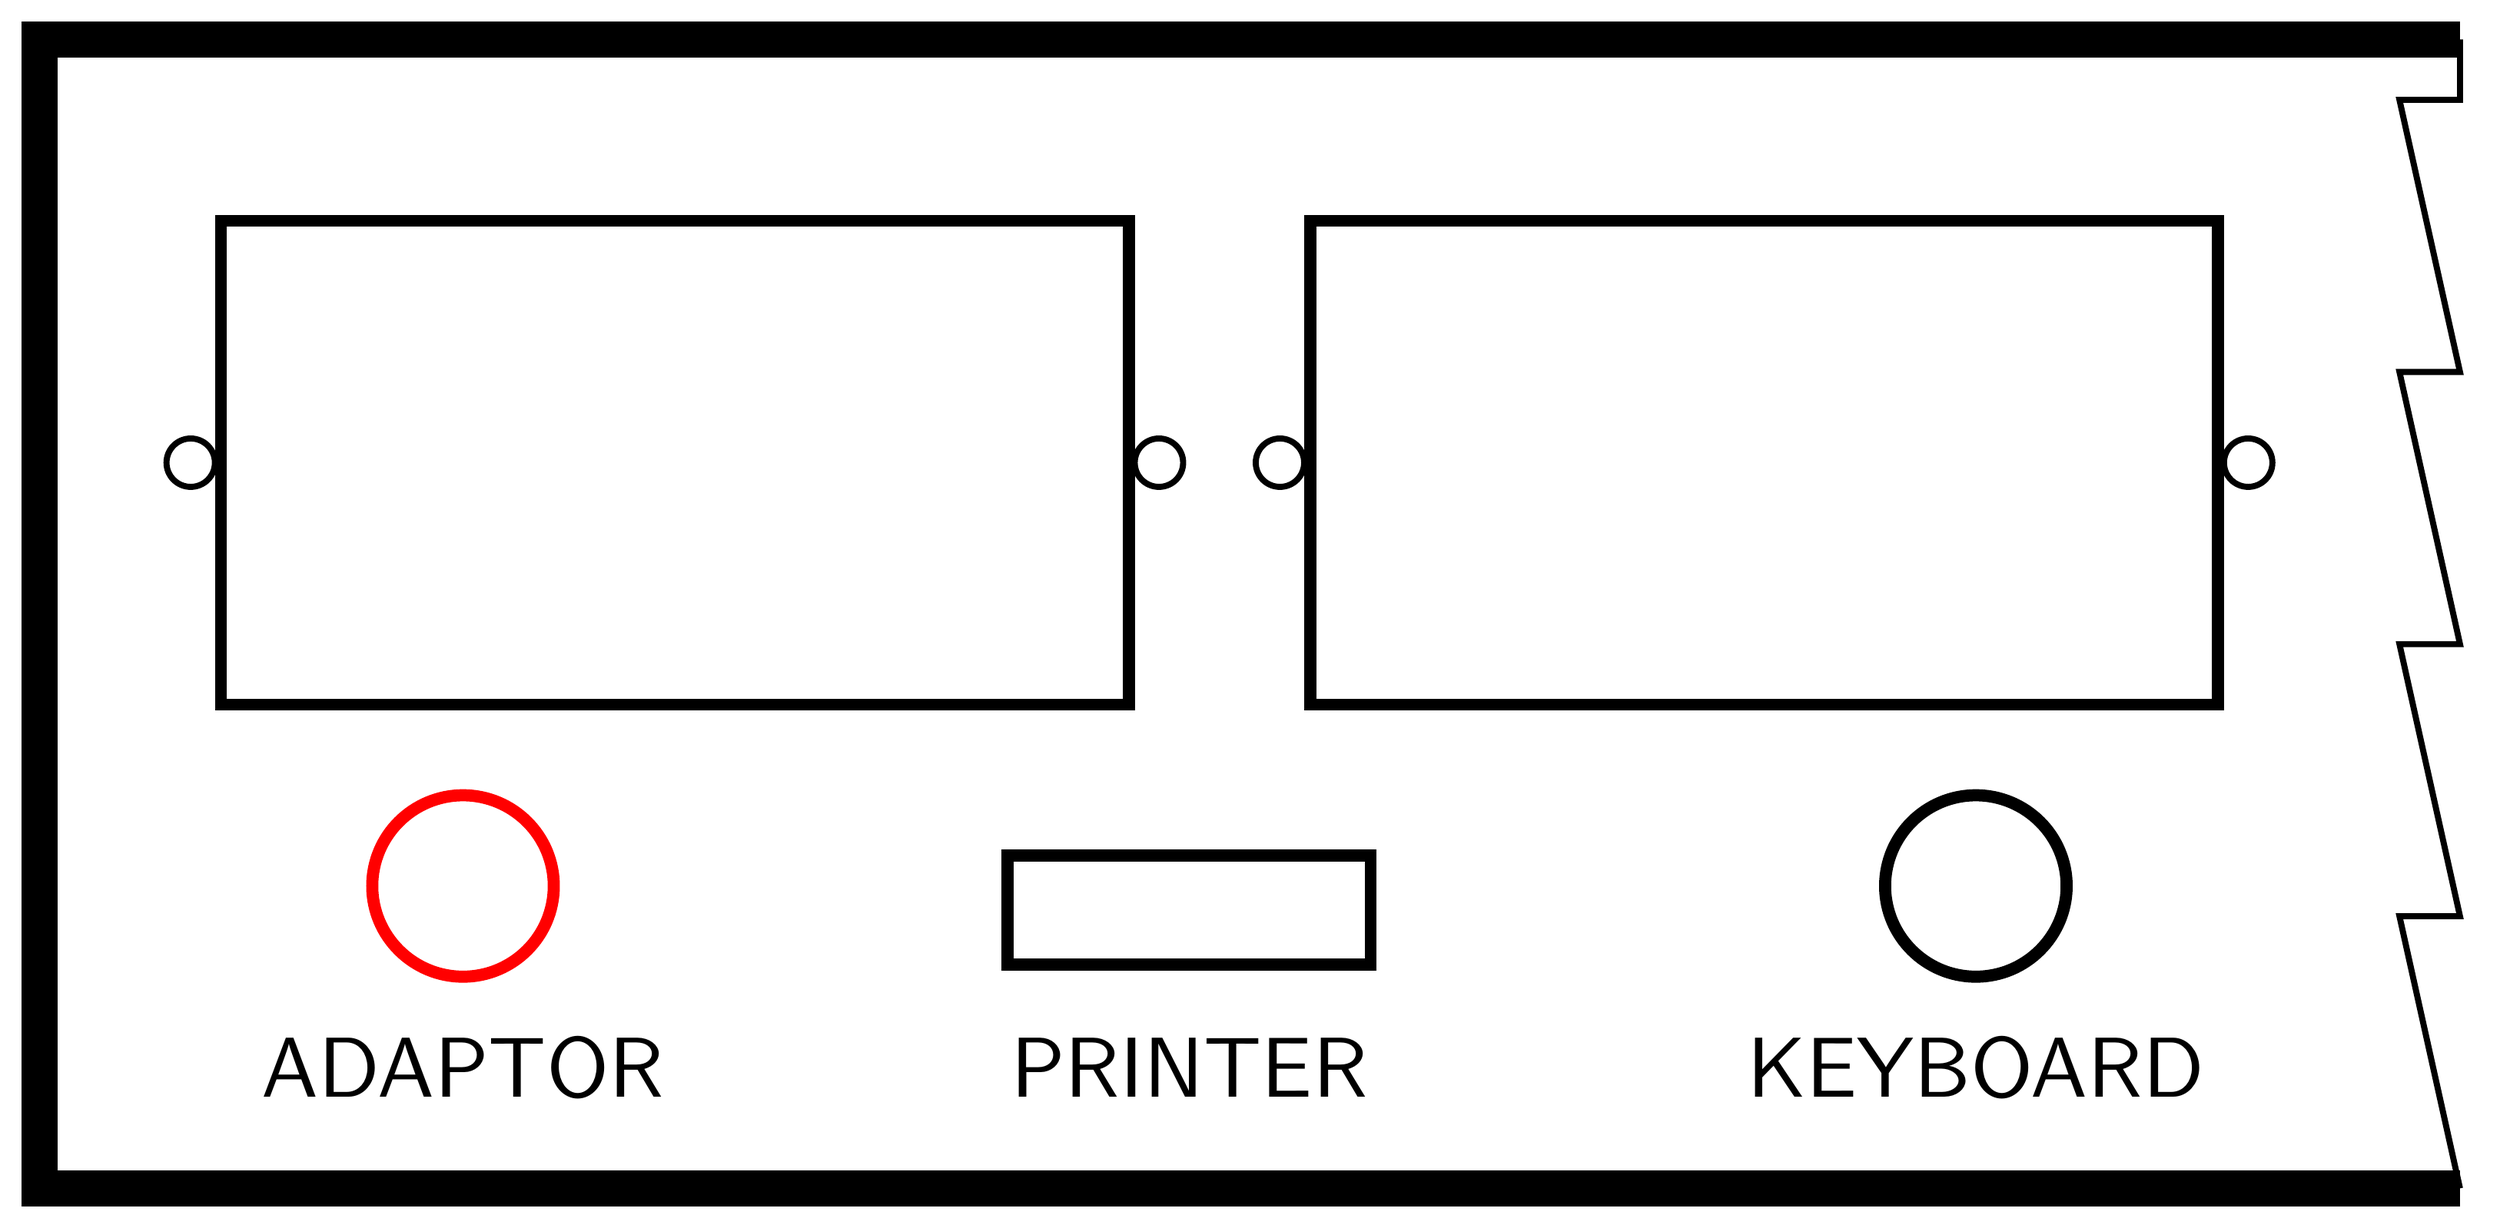
\begin{tikzpicture}[font=\sffamily]
				\draw[line width=6mm] (40,19) -- ++(-40,0) -- ++(0,-19) -- ++(40,0);
				\draw[line width=1mm,decorate,decoration={saw,segment length=45mm,amplitude=10mm}] (40,0) -- ++(0,19);
				\draw[line width=2mm,fill=white] (3,8) rectangle (18,16);
				\draw[line width=2mm,fill=white] (21,8) rectangle (36,16);
				\draw[line width=1mm,fill=white] (2.5,12) circle (4mm);
				\draw[line width=1mm,fill=white] (18.5,12) circle (4mm);
				\draw[line width=1mm,fill=white] (20.5,12) circle (4mm);
				\draw[line width=1mm,fill=white] (36.5,12) circle (4mm);

				\draw[line width=2mm,color=red,fill=white] (7,5) circle (15mm);
				\draw[line width=2mm,fill=white] (32,5) circle (15mm);
				\node[black,scale=4] at (7,2) {ADAPTOR};
				\node[black,scale=4] at (32,2) {KEYBOARD};
				\draw[line width=2mm,fill=white] (16,3.7) rectangle (22,5.5); \node[black,scale=4,] at (19,2) {PRINTER};
			\end{tikzpicture}
		}
		\caption[Adaptor port position.]{NABU Personal Computer \texttt{ADAPTOR} port.}
		\label{fig:backplane}
	\end{center}
\end{figure}

\begin{figure}[h!]
	\begin{center}
		\scalebox{0.175}{
			\begin{tikzpicture}[font=\sffamily]
				\draw[line width=6mm] (10,10) circle (8cm);
				\draw[line width=1mm] (10,10) circle (7cm);
				\fill[fill=white] (9,3.5) rectangle (11,2.8);
				\begin{scope}
					\clip (8.8,3.05) rectangle (11.2,6);
					\draw[line width=1mm] (10,3) circle (1cm);
				\end{scope}
				\foreach \p\k\n\m\r [count=\q from 0] in {{RXD+}/1/10/5/190,{RXD--}/4/13.4/6.4/160,{}/2/15/10/0,{T/R+}/5/13.4/13.6/20,{T/R--}/3/10/15/350} {
					\ifthenelse{\k=2}{}{
						\ifthenelse{\q>1}{\def\a{right}\def\w{1.75cm}}{\def\a{left}\def\w{2.25cm}}
						\draw[line width=1mm,red] (\m,\n) -- ++(\r:6cm) node[black,scale=4,text width=\w,align=\a]{\p};
					}
					\draw[line width=1mm,fill=white] (\m,\n) circle (7mm) node[scale=3,gray,yshift=-1.5em]{\k};
				}
			\end{tikzpicture}
		}
		\caption[DIN-5 male connector pinouts.]{DIN-5 male connector (solder side).}
		\label{fig:din5}
	\end{center}
\end{figure}

\section{DB-9 end of the cable}
\begin{enumerate}
	\item Solder the pins on the \underline{female} DB-9 connector as shown in Figure \ref{fig:dsub9}.  Note that the pin numbers shown in the diagram are for the solder side of the connector.
\end{enumerate}

\begin{figure}[h!]
  \begin{center}
	\scalebox{0.2}{
		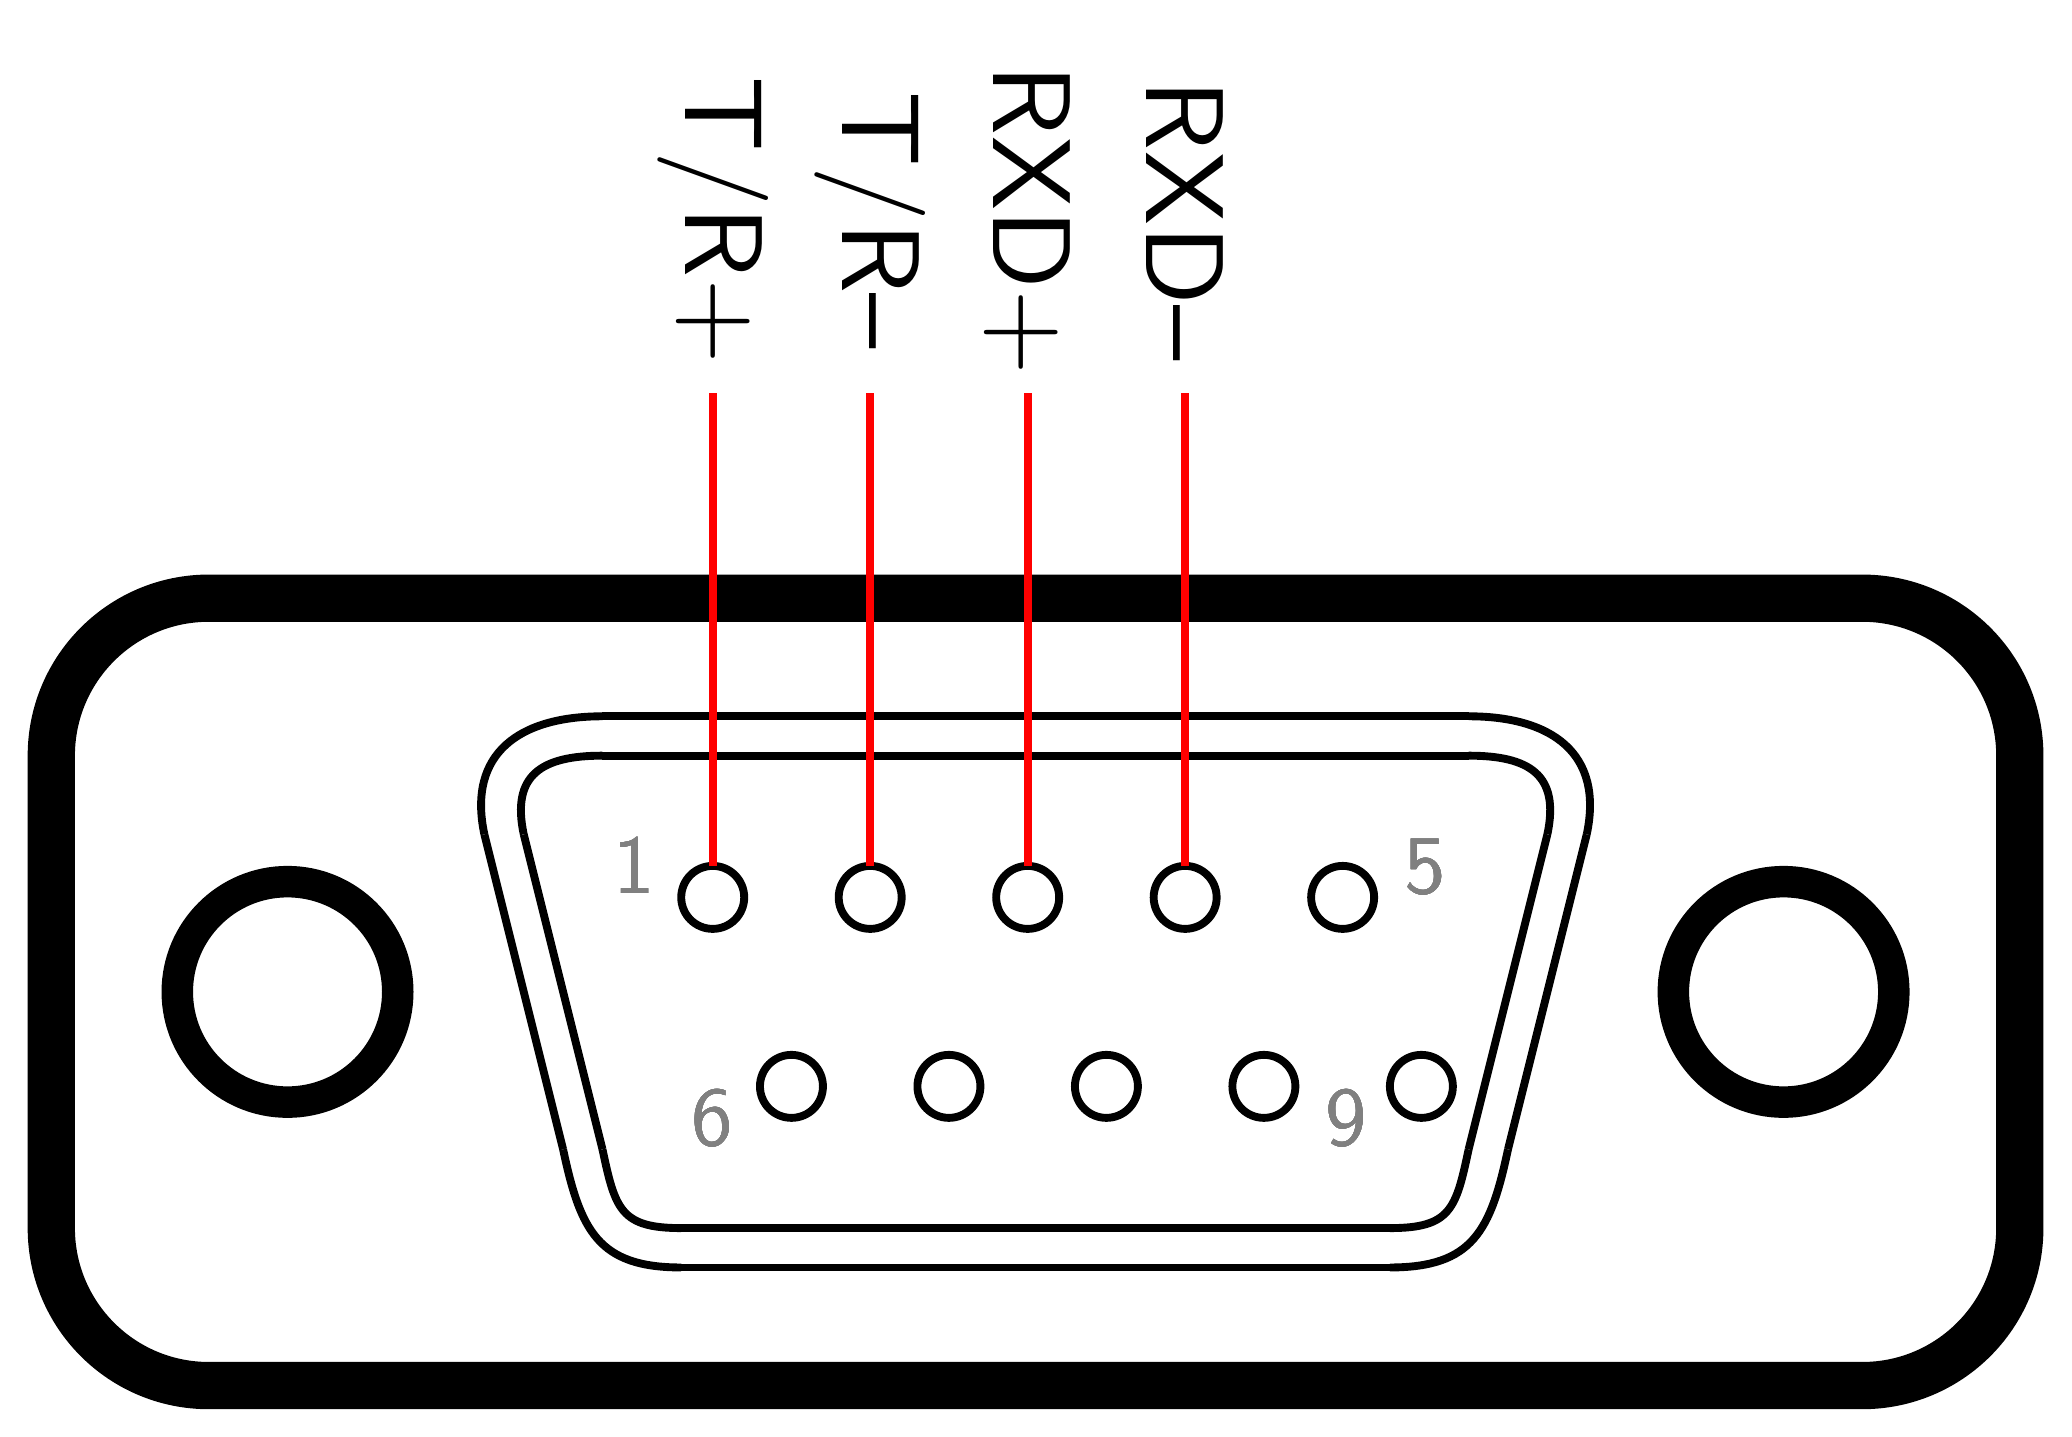
\begin{tikzpicture}[font=\sffamily]
			\draw[rounded corners=2cm,line width=6mm] (0, 0) rectangle (25,10) {};

			\draw[line width=4mm] (3,5) circle (1.4cm);
			\draw[line width=4mm] (22,5) circle (1.4cm);

			\draw[line width=1mm] (7,8) -- (18,8);
			\draw[line width=1mm] (8,2) -- (17,2);
			\draw[line width=1mm] (6,7) -- (7,3);
			\draw[line width=1mm] (19,7) -- (18,3);
			\draw[line width=1mm] (6,7) to[out=102,in=180,distance=22] (7,8);
			\draw[line width=1mm] (7,3) to[out=-78,in=180,distance=22] (8,2);
			\draw[line width=1mm] (17,2) to[out=0,in=-102,distance=22] (18,3);
			\draw[line width=1mm] (19,7) to[out=78,in=0,distance=22] (18,8);

			\draw[line width=1mm] (7,8.5) -- (18,8.5);
			\draw[line width=1mm] (8,1.5) -- (17,1.5);
			\draw[line width=1mm] (5.5,7) -- (6.5,3);
			\draw[line width=1mm] (19.5,7) -- (18.5,3);
			\draw[line width=1mm] (5.5,7) to[out=102,in=180,distance=30] (7,8.5);
			\draw[line width=1mm] (6.5,3) to[out=-78,in=180,distance=30] (8,1.5);
			\draw[line width=1mm] (17,1.5) to[out=0,in=-102,distance=30] (18.5,3);
			\draw[line width=1mm] (19.5,7) to[out=78,in=0,distance=30] (18,8.5);

			\foreach \p\k [count=\q from 0] in {{T/R+}/{},{T/R--}/{},{RXD+}/{},{RXD--}/{},{}/{}} {
				\draw[line width=1mm] (8.4+\q*2,6.2) circle (4mm);
				\ifthenelse{\q<4}{\draw[line width=1mm] (9.4+\q*2,3.8) circle (4mm);	}{}
				\foreach \x in \p {
					\draw[line width=1mm,red] (8.4+\q*2,6.6) -- ++(0,6);
					\draw (8.4+\q*2,14.8) node[rotate=-90,scale=4]{\p};
				}{}
				\foreach \x in \k {
					\draw[line width=1mm,red] (9.4+\q*2,3.4) -- ++(0,-6);
					\draw (9.4+\q*2,-4.8) node[rotate=-90,scale=4,text width=1cm]{\k};
				}
				\draw (7.4,6.6) node[scale=3,gray]{1};
				\draw (17.45,6.6) node[scale=3,gray]{5};
				\draw (8.4,3.4) node[scale=3,gray]{6};
				\draw (16.45,3.4) node[scale=3,gray]{9};
			}
		\end{tikzpicture}
	}
	\caption[DB-9 female connector pinouts.]{DB-9 female connector (solder side).$^2$}
	\label{fig:dsub9}
  \end{center}
\end{figure}
%\begin{figure}[t!]
%	\begin{center}
%		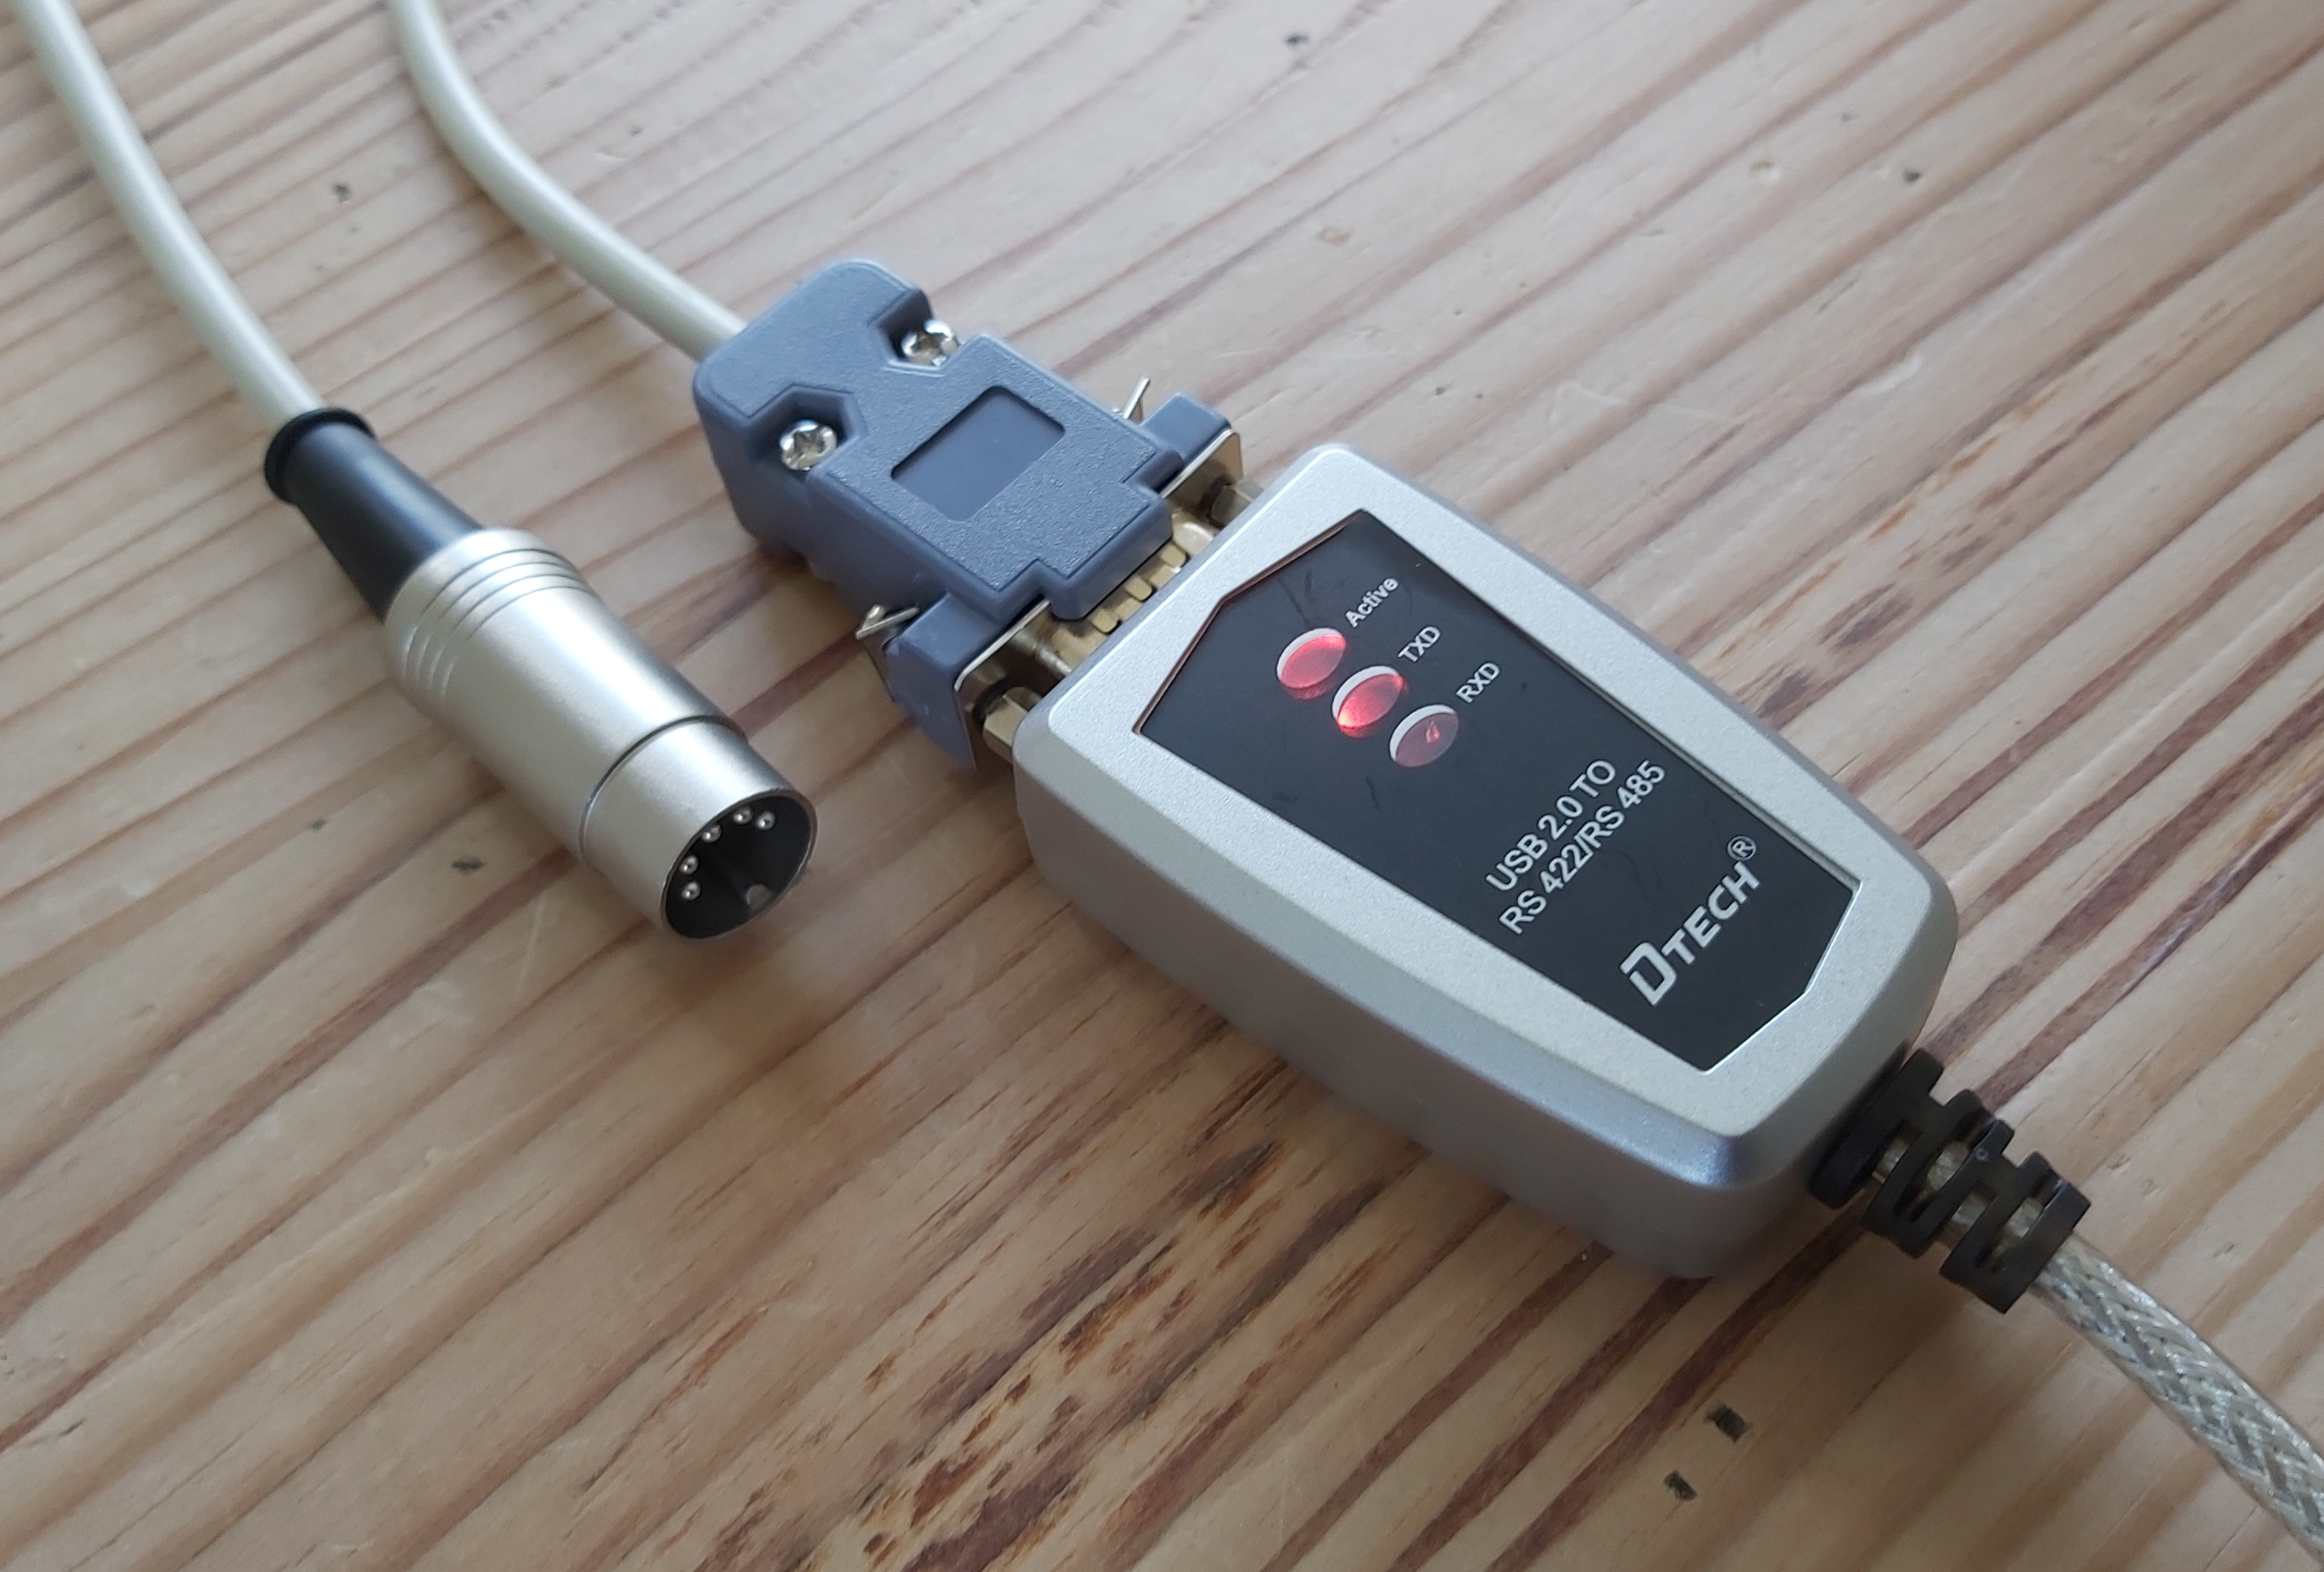
\includegraphics[width=\columnwidth]{images/rs422-image-1.jpg}
%		\caption{DB-9 to DIN-5 Network Adaptor assembly.}
%	\end{center}
%\end{figure}
